\section{Auswertung}
\subsection{Ersatzschaltbild Transformator}
\begin{enumerate}[label=\alph*)]
	\item Zeichnen Sie das vollständige einphasige Ersatzschaltbild (Sternschaltung) des
	      Transformators.
	      \begin{figure}[h!]
		      \begin{center}
			      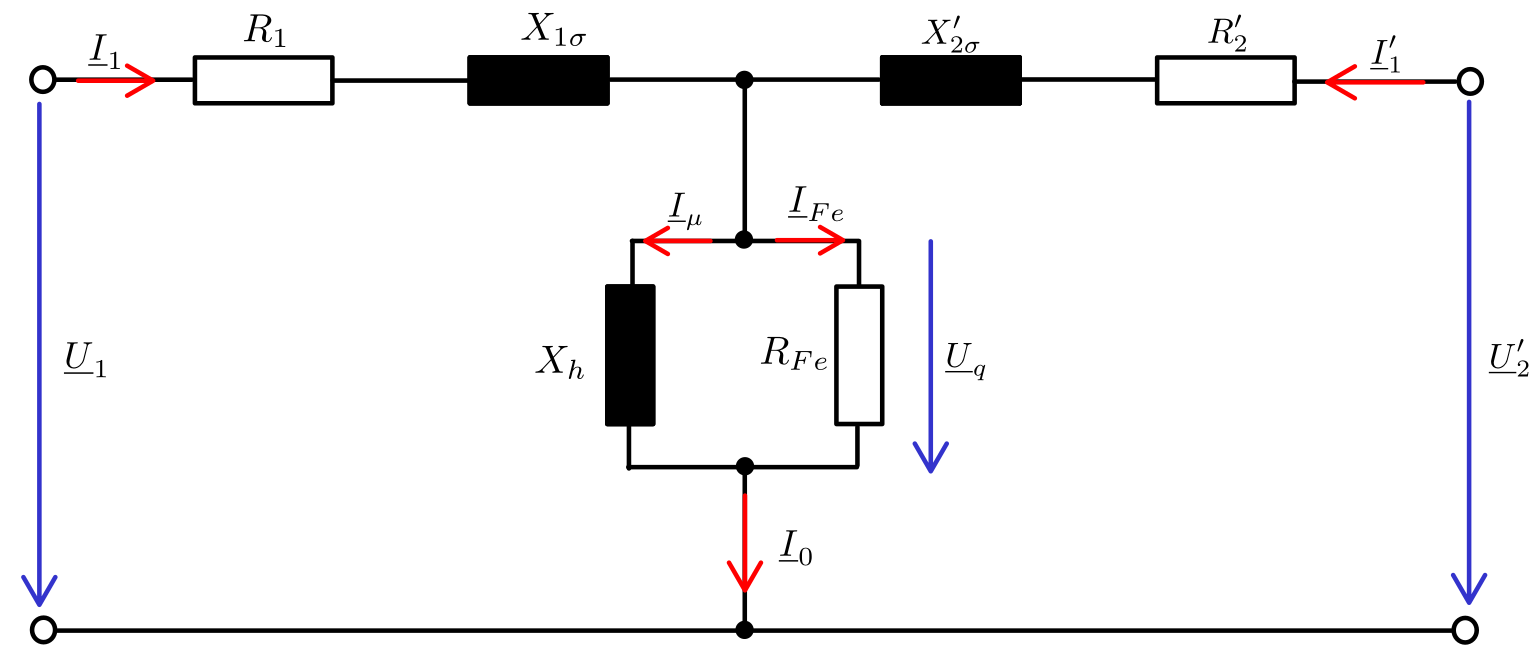
\includegraphics[width=0.95\textwidth]{img/4.1.1.1}
		      \end{center}
		      \caption{}\label{img:4.1.1.1}
	      \end{figure}

	\item Bestimmen Sie die Leistung im Leerlauf auf der Primärseite nach Gleichung (16).
	      \begin{align*}
		      \underline S & = \underline U_{12} \cdot \underline I_1^* + \underline U_{32}\cdot \underline I_3^*   \\
		      \underline S & = \underline U_{12} \cdot \underline I_1^* + \underline U_{23}^*\cdot \underline I_3^* \\
		      \underline S & = 395\ V \cdot e^{j0^\circ} \cdot 0.45\ A \cdot e^{-(-j120^\circ)} +
		      393\ V \cdot e^{-(-j120)^\circ}\cdot 0.45\ A \cdot e^{-(j45^\circ)}                                   \\
		      \underline S & = -43,1\ W + j324,76\ var = 327,6\ VA\cdot e^{j97,6^\circ}
	      \end{align*}

	\item Bestimmen Sie die Wirkleistung im Kurzschlussfall auf der Sekundärseite nach
	      Gleichung (16). Gehen Sie dabei von einem symmetrischen System aus.
	      \begin{align*}
		      \underline S & = \underline U_{12} \cdot \underline I_1^* + \underline U_{32}\cdot \underline I_3^*   \\
		      \underline S & = \underline U_{12} \cdot \underline I_1^* + \underline U_{23}^*\cdot \underline I_3^* \\
		      \underline S & = 12.5\ V \cdot e^{j0^\circ} \cdot 7,4\ A \cdot e^{-(-j50^\circ)}
		      + 12\ V \cdot e^{-(-j120^\circ)}\cdot 7,5\ A \cdot e^{-(j70^\circ)}                                   \\
		      \underline S & = 113\ W+j 135,\ var = 177\ VA \cdot e^{j50^\circ}                                     \\
		      P            & = 113\ W
	      \end{align*}

	\item Ermitteln Sie die Daten des vollständigen Ersatzschaltbildes des Transformators
	      mit der Annahme $X_{1\sigma} = X'_{2\sigma} \text{ sowie } R_1 = R'_2$.
	      \begin{align*}
		      \underline Z_K & = R_K + JX_{K}                                                                                 \\
		      \underline Z_K & = R_1 + R'_2 + J(X_{1\sigma} + X2'_{2\sigma})                                                  \\
		      \underline Z_K & = 2R_1 + J2X_{1\sigma}                                                                         \\
		      \underline Z_K & = \frac{\underline \Delta U}{\underline I_1} = \frac{395\ V\cdot e^{j0} - 12,5\ V\cdot e^{j0}}
		      {7,3\ A \cdot e^{-j50^\circ}}                                                                                   \\
		      \underline Z_K & = 33,7 \Omega + j40,1 \Omega                                                                   \\
		      R_1 = R'_2     & = \frac {Re\{\underline Z_K\}}{2} = \frac{33,7\ \Omega}{2} = 16,85\ \Omega                     \\
		      X_{1\sigma}    & = X'_{2\sigma} = \frac {Im\{\underline Z_K\}}{2} = \frac{40,1\ \Omega}{2} = 20,05\ \Omega      \\
	      \end{align*}

	\item Berechnen Sie anhand des Kurzschlussversuches die relative Kurzschlussspannung
	      des Transformators.
	      \begin{align*}
		      u_k & = \frac{U_K}{U_N}      \\
		      u_k & = \frac{12\ V}{400\ V} \\
		      u_k & = 3\%
	      \end{align*}

\end{enumerate}
\subsection{Symmetrische Drehstromlast}
\begin{enumerate}[label=\alph*)]

	\item Berechnen Sie aus den Messwerten nach 3.2(b) die gemittelten Größen $U_m, I_m
		      \text{ und } \varphi_m$ (siehe Versuch E2-4), den Leistungsfaktor $\lambda =
		      \cos(\varphi_m)$, die Leistungen $S, P \text{ und } Q$ jeweils für die Primär-
	      und die Sekundärseite.\\ \ \\
	      \begin{center}
		      \begin{align*}
			      \varphi_{\Delta} & = \varphi_{U} - \varphi_{I}                             \\
			      S                & = \sqrt{3}\cdot U_M\cdot I_M                            \\
			      P                & = \sqrt{3}\cdot U_M\cdot I_M\cdot\cos(\varphi_{\Delta}) \\
			      Q                & = \sqrt{3}\cdot U_M\cdot I_M\cdot\sin(\varphi_{\Delta}) \\
			      \lambda          & = \frac{|P|}{S}                                         \\
		      \end{align*}
	      \end{center}

	      \textbf{Primärseite}\\ \ \\

	      \begin{tcolorbox}[colback=gray!30,
			      colframe=black,
			      width=0.9\textwidth,
		      ]
		      \parbox{\textwidth}{

			      \begin{minipage}{0.5\textwidth}
				      \textbf{Spannung}:
				      \begin{align*}
					      U_{M.pri} & = \frac{U_{12} + U_{23} + U_{31}}{3} \\
					      U_{M.pri} & = \frac{378\ V + 371\ V + 372\ V}{3} \\
					      U_{M.pri} & = 373,67\ V                          \\
				      \end{align*}
			      \end{minipage}\hfill
			      \begin{minipage}{0.5\textwidth}
				      \textbf{Strom}:
				      \begin{align*}
					      I_{M.pri} & = \frac{I_{12} + I_{23} + I_{31}}{3} \\
					      I_{M.pri} & = \frac{7\ A + 7\ A + 7\ A}{3}       \\
					      I_{M.pri} & = 7\ A                               \\
				      \end{align*}
			      \end{minipage}
		      }
	      \end{tcolorbox}

	      \textbf{Sekundärseite}\\ \ \\

	      \begin{tcolorbox}[colback=gray!30,
			      colframe=black,
			      width=0.9\textwidth,
		      ]
		      \parbox{\textwidth}{

			      \begin{minipage}{0.5\textwidth}
				      \textbf{Spannung}:
				      \begin{align*}
					      U_{M.sec} & = \frac{U_{12} + U_{23} + U_{31}}{3} \\
					      U_{M.sec} & = \frac{378\ V + 371\ V + 358\ V}{3} \\
					      U_{M.sec} & = 354\ V                             \\
				      \end{align*}
			      \end{minipage}\hfill
			      \begin{minipage}{0.5\textwidth}
				      \textbf{Strom}:
				      \begin{align*}
					      I_{M.sec} & = \frac{I_{12} + I_{23} + I_{31}}{3} \\
					      I_{M.sec} & = \frac{7\ A + 7\ A + 6,7\ A}{3}     \\
					      I_{M.sec} & = 6,9\ A                             \\
				      \end{align*}
			      \end{minipage}
		      }
	      \end{tcolorbox}
	      \begin{table}[h!]
		      \caption{Brechnung der Eingangsseite Yy5 Symmetrischelast}
		      \centering
		      \begin{tabular}{lrrrrr}
			      \hline
			      Impedanzen & $\varphi$    & $S$    & $P$      & $Q$      & $\lambda$ \\ \hline
			      $Z_1$      & $65^\circ$   & $4,53$ & $-2,55$  & $ 3,75 $ & $0,56$    \\
			      $Z_2$      & $65^\circ$   & $4,53$ & $-2,55 $ & $ 3,75$  & $0,56$    \\
			      $Z_3$      & $67^\circ  $ & $4,53$ & $-2,35$  & $ -3,88$ & $0,52$    \\ \hline
		      \end{tabular}
	      \end{table}
	      \begin{table}[h!]
		      \caption{Brechnung der Ausgangsseite Yy5 Symmetrischelast}
		      \centering
		      \begin{tabular}{lrrrrr}
			      \hline
			      Impedanzen & $\varphi$     & $S$    & $P$      & $Q$     & $\lambda$ \\ \hline
			      $Z_1$      & $-43^\circ$   & $4,33$ & $-1,83$  & $-3,82$ & $0,43$    \\
			      $Z_2$      & $-43^\circ$   & $4,33$ & $-1,83 $ & $-3,82$ & $0,43$    \\
			      $Z_3$      & $-43^\circ  $ & $4,33$ & $-1,83$  & $-3,82$ & $0,43$    \\ \hline
		      \end{tabular}
	      \end{table}

	\item Berechnen Sie die Verlustleistung des Transformators sowie den Wirkungsgrad mit
	      den Ergebnissen aus 4.2(a).
	      \begin{figure}[h!]
		      \begin{center}
			      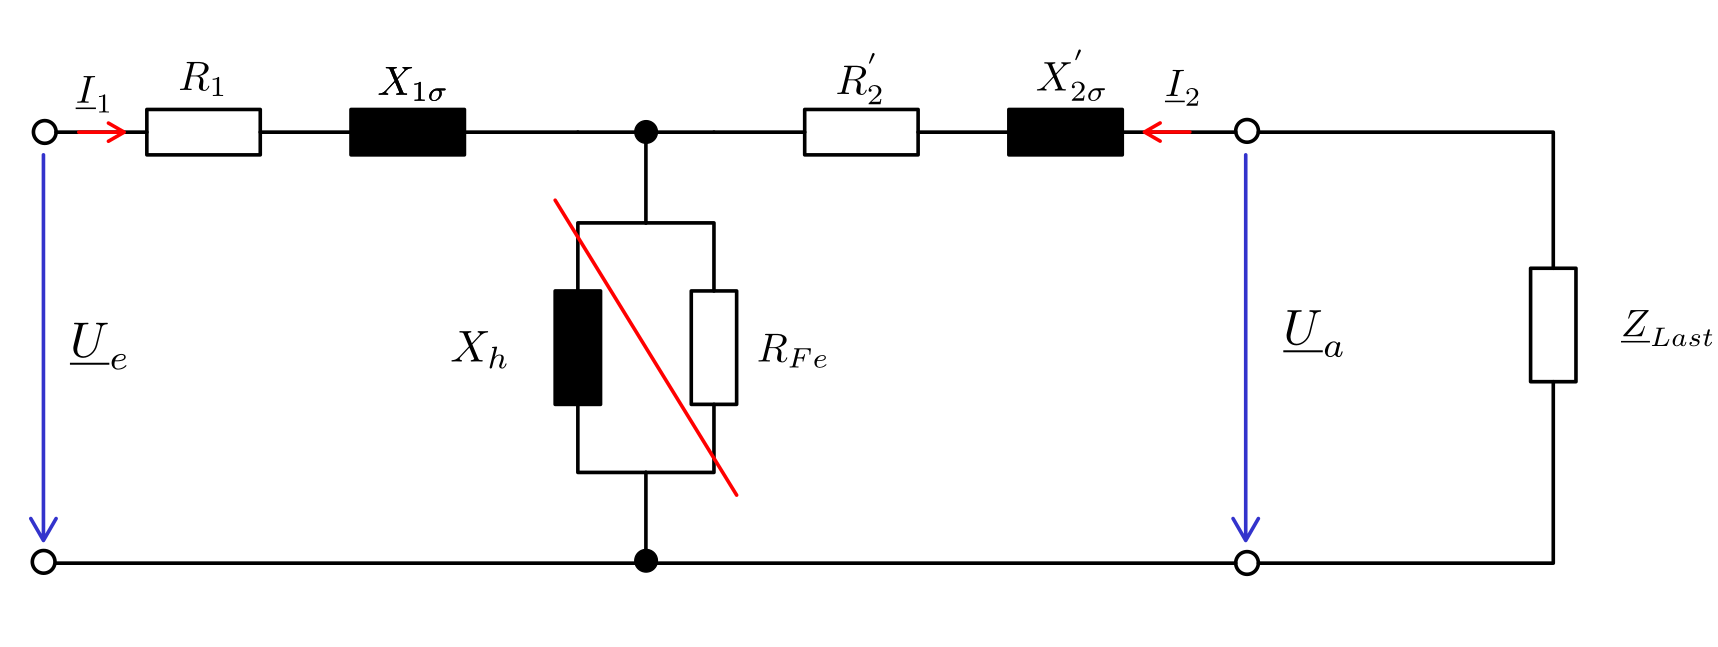
\includegraphics[width=0.8\textwidth]{img/4.2.2.1}
		      \end{center}
		      \caption{ESP für den Transformator im Lastbetrieb}\label{img:4.2.2.1}
	      \end{figure}

		  
	      \begin{align*}
		      \eta & = \frac{P_{ab}}{P_{zu}}                                                                                                       \\
		      \eta & = \frac{\sqrt{3}\cdot U_{M.sec}\cdot I_{M.sec}\cdot \cos(\varphi)}{\sqrt{3}\cdot U_{M.pri}\cdot I_{M.pri}\cdot \cos(\varphi)} \\
		      \eta & = \frac{354\ V\cdot 7\ A}{373,6\ V\cdot 6,7\ A}                                                                               \\
		      \eta & = 0,989
	      \end{align*}

	      \begin{figure}[h!]
		      \begin{center}
			      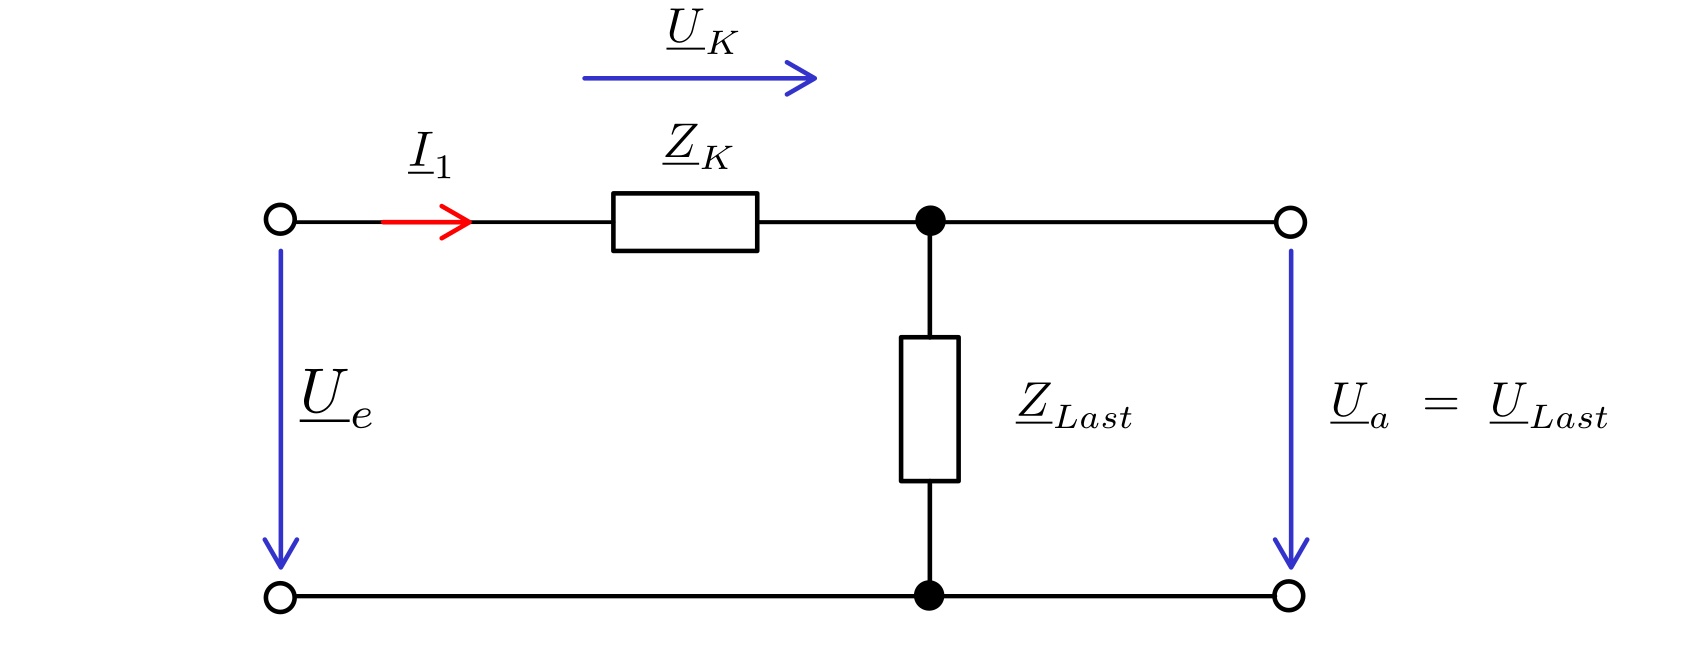
\includegraphics[width=0.8\textwidth]{img/4.2.2.2}
		      \end{center}
		      \caption{Vereinfachtest ESP für den Transformator im Lastbetrieb}\label{img:4.2.2.2}
	      \end{figure}
	      \begin{align*}
		      0     & = -\underline{U}_{e}+\underline{U}_{K}+\underline{U}_{a} \\
		      U_{K} & = U_{e}-U_{a}                                            \\
		      U_{K} & = 373\ V - 354\ V                                        \\
		      U_{K} & = 19\ V
	      \end{align*}
	      

	\item Bestimmen Sie die Verlustleistung für 3.2(b) nach 2.1(d) und vergleichen Sie
	      das Ergebnis mit dem Wert aus 4.2(b). Begründen Sie Ihre Beobachtungen.

	      \begin{minipage}[r]{0.5\linewidth}
		      \begin{align*}
			      P_{FE} & = P_0\ (\frac{U}{U_N})^2              \\
			      P_{FE} & = -43,1\ W\ (\frac{373\ V}{400\ V})^2 \\
			      P_{FE} & = -37,477\ W
			      \\
			      \\
			      P_{Cu} & = P_K\ (\frac{I}{I_N})^2              \\
			      P_{Cu} & = 113\ W\ (\frac{7\ A}{7,2\ A})^2     \\
			      P_{Cu} & = 106,909\ W
		      \end{align*}
	      \end{minipage}
	      \begin{minipage}[l]{0.5\linewidth}
		      \begin{align*}
			      P_{V} & = P_{FE} \ +\ P_{Cu}                                  \\
			      P_{V} & = -37,477\ W + 106,909\ W                             \\
			      P_{V} & = 69,33\ W
			      \\
			      \\
			      \eta  & = 1-\frac{P_{v}}{S}                                   \\
			      \eta  & = 1- \frac{69,33\ W}{\sqrt{3}\cdot 354\ V\cdot 7\ A } \\
			      \eta  & = 0,9838
		      \end{align*}
	      \end{minipage}

	\item Berechnen Sie aus den Messwerten nach 3.2(b) und dem Übersetzungsverhältnis ü
	      den relativen Spannungsfall $\Delta u'_2$!\\ \ \\

	      \begin{minipage}[r]{0.5\linewidth}
		      \begin{align*}
			      U_1 & = ü\cdot U_2            \\
			      ü   & = \frac{U_1}{U_2}       \\
			      ü   & = \frac{373\ V}{354\ V} \\
			      ü   & = 1,053                 \\
			      ü   & \approx 1
		      \end{align*}
	      \end{minipage}
	      \begin{minipage}[l]{0.5\linewidth}
		      \begin{align*}
			      I_2 & = ü\cdot I_1          \\
			      ü   & = \frac{I_2}{I_1}     \\
			      ü   & = \frac{6,9\ A}{7\ A} \\
			      ü   & = 0,985               \\
			      ü   & \approx 1
		      \end{align*}
	      \end{minipage}

	\item Bestimmen Sie anhand der Formeln (11) - (13) den relativen Spannungsabfall für
	      3.2(b).

	      \begin{align*}
		      \Delta u'_2 & = \frac{U_1\ -\ U'_2}{U_1}                       \\
		      \Delta u'_2 & = \frac{373\ V -\frac{373\ V}{\sqrt{3}}}{373\ V} \\
		      \Delta u'_2 & = 0,422                                      \\
	      \end{align*}
	      \begin{align*}
		      U_l         & = I_1(R_K\cos(\varphi_2)+X_K\sin(\varphi_2))                              \\
		      U_l         & = 7\ A\ (33,7\ \Omega\ \cos(-46^\circ)\ +\ 40,1\ \Omega\ \sin(-46^\circ)) \\
		      U_l         & = -38,728\ V                                                              \\
		      \\
		      U_q         & = I_1(R_K\cos(\varphi_2)+X_K\sin(\varphi_2))                              \\
		      U_q         & = 7\ A\ (33,7\ \Omega\ \sin(-46^\circ)\ +\ 40,1\ \Omega\ \cos(-46^\circ)) \\
		      U_q         & = 24,592\ V                                                               \\
		      \\
		      \Delta u'_2 & = 1+\frac{U_l}{U_1} - \sqrt{1-\frac{U_q}{U_1}}                            \\
		      \Delta u'_2 & = 1+\frac{-38,728\ V}{373,67\ V} - \sqrt{1-\frac{24,592\ V}{373,67\ V}}   \\
		      \Delta u'_2 & = 0,100\ 336
	      \end{align*}

	\item Vergleichen Sie die primär- und sekundärseitigen Spannungen und Ströme aus
	      3.2(b) und 3.2(c) miteinander.

\end{enumerate}
